\section{Premier raffinement}

\subsection{Analyse}
Dans cette partie, on introduit la piste pour évoluer vers un modèle plus concret. On peut ainsi spécifier le nombre d'avions se trouvant sur la piste en vue  d'un décollage et après un atterrissage ainsi que le nombre d'avions sur le tarmac.
Ce fait implique un "raffinement" des exigences environnementales ; on doit avoir un capteur capable de compter les avions au décollage et un capteur pour les avions à l'atterrissage. Ce qui donne les exigences modifiées suivantes :


\begin{table} [H]
	\centering
\rowcolors{2}{gray!65}{white}
\begin{tabu}{|[2pt] p{1.7cm} | [2pt]p{15cm}|[2pt]}
	
	\tabucline[2pt]{-} \rowcolor{yellow}
	\Centering	\textbf{Label}& \Centering \textbf{Exigence}  \\ \tabucline[2pt]{-}
	
	\hline 
	FON-1&Le contrôleur doit autoriser les avions à décoller et atterrir  \\ 
	\hline 
	FON-1.1& \textcolor{red}{Le contrôleur doit fonctionner indéfiniment une fois lancé.}  \\ 
	\hline 
	FON-2	& Le nombre d'avions immobilisés sur le tarmac est limité à 20 y compris ceux en attente de décollage\textcolor{red}{mais doit rester positif} \\ 
	\hline 
	FON-3& Des avions entrent sur et quittent la piste d'atterrissage décollage  \\ 
	\hline 
	FON-4& Des avions entrent sur le tarmac et le quittent  \\ 
	\hline 
	FON-5& La piste ne peut être occupée par un avion au décollage et un avion à l'atterrissage en même temps. \\ 
	\hline 
	FON-6& Le nombre de décollages ou atterrissages successifs n'est pas limité   \\ 
	\hline 
	FON-7& Le contrôleur doit fixer et délivrer les clearances à l'avance   \\ 
	\hline 
	FON-8& Le contrôleur ne doit autoriser l'avion qu'après l'envoi de son identifiant    \\ 
	\hline
	FON-9& Le contrôleur doit soit refuser, soit accepter, soit mettre en attente l'avion demandeur   \\ 
	\hline
	FON-10& Le contrôleur doit refuser la clearance après 10mn de mise en attente.   \\ 
	\hline 
	ENV-1 &Tout avion se dirigeant vers la piste doit avoir une autorisation de décoller \\ 
	\hline 
	ENV-2 &\textcolor{blue}{Le système est muni d'un capteur qui permet de compter les avions sur la piste à l'atterrissage et un capteur pour les avions sur la piste au décollage.} \\ 
	\hline 
	ENV-3 &Le système est muni d'un capteur qui permet de compter les avions sur la tarmac \\ 
	\tabucline[2pt]{-}
\end{tabu} 
\caption{Tableau des exigences V3}
\end{table}

\begin{figure}[H]
	\begin{center}	
		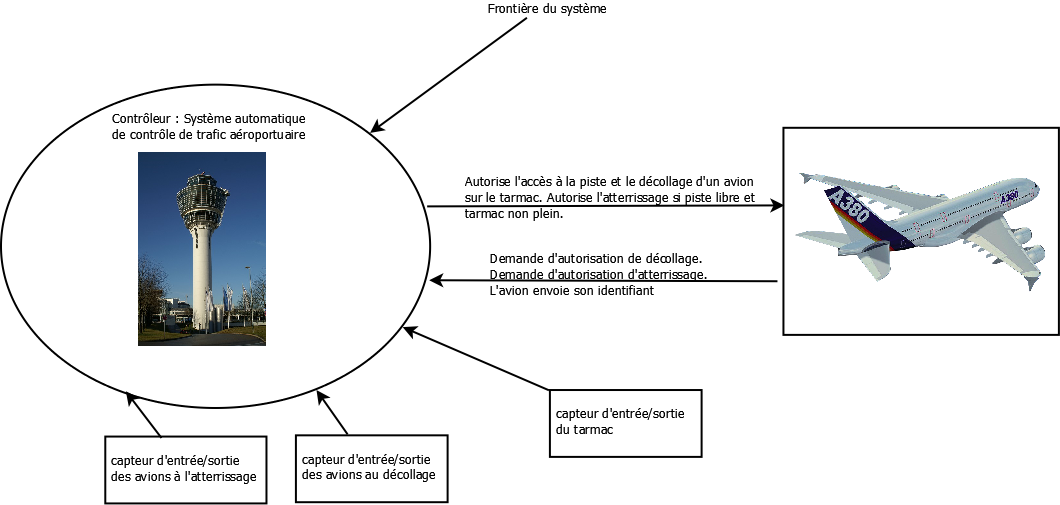
\includegraphics[scale=0.3]{images/1/env2}
		\caption{Environnement du système : version 2}
		\label{ctx}
	\end{center}
\end{figure}
\begin{figure}[H]
	\begin{center}	
		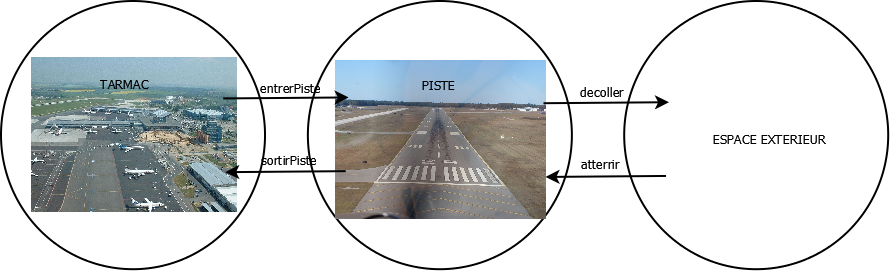
\includegraphics[scale=0.4]{images/1/raf1}
		\caption{Premier raffinement du système : piste et tarmac sont différenciés}
		\label{raf1}
	\end{center}
\end{figure}
\paragraph{}
Contrairement à ce qui se passe dans la réalité, les spécifications laissent la possibilité d'avoir au même moment plusieurs avions sur la piste au décollage ou à l'atterrissage dès lors qu'on ne mélange pas les décollages et atterrissages.
La piste est, à un instant donné, en sens unique.


%\subsection{raffinement de l'état du système clos}
%\begin{figure}[H]
%	\begin{center}	
%		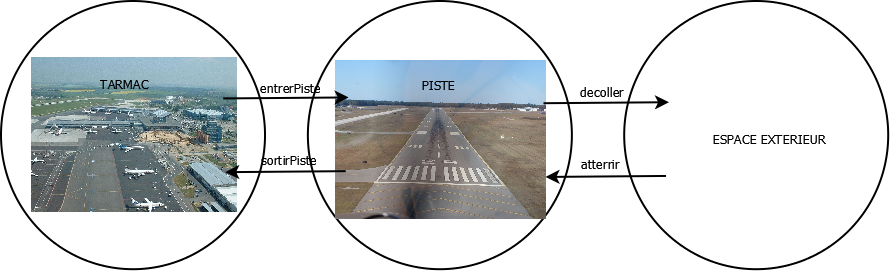
\includegraphics[scale=0.4]{images/1/raf1}
%		\caption{Premier raffinement du système : la piste et le tarmac sont différenciés}
%		\label{raf1}
%	\end{center}
%\end{figure}

\subsection{Contexte}
Le CONTEXTE n'est pas modifié. La constante ntmax du système caractérise l'état statique du système concret associé à ce premier raffinement.

\begin{figure}[H]
	\begin{center}	
		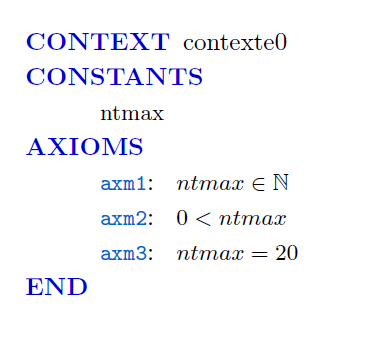
\includegraphics[scale=1]{images/1/ctx1}
		\caption{Contexte premier raffinement}
		\label{ctx1}
	\end{center}
\end{figure}

\subsection{Glue}Ces variables vérifient nbAvionsDecollage + nbAvionsAtterrissage + nbAvionsTarmac = nt. C'est l'invariant de "glue" qui fait le lien entre les 3 variables concrètes et la variable abstraite nt.

\subsection{Convergence des nouveaux events}

On définit un variant entier naturel, en l'occurrence, $nbAvionsTarmac + 2 ∗ nbAvionsAtterrissage$ dont on a vérifié qu'il est bien décrémenté par les deux nouveaux events introduits: $entrerPiste$ et $sortirPiste$ pour éviter qu'ils ne soient indéfiniment activés avec pour conséquence une interdition des décollages et atterrissages.

\subsection{Machine}
 On définit une nouvelle machine nommée "raffinement1" pour prendre en compte les nouvelles variables. La Machine raffinement1 est obtenue par raffinage de la machine0.
 \begin{figure}[H]
 	\begin{center}	
 		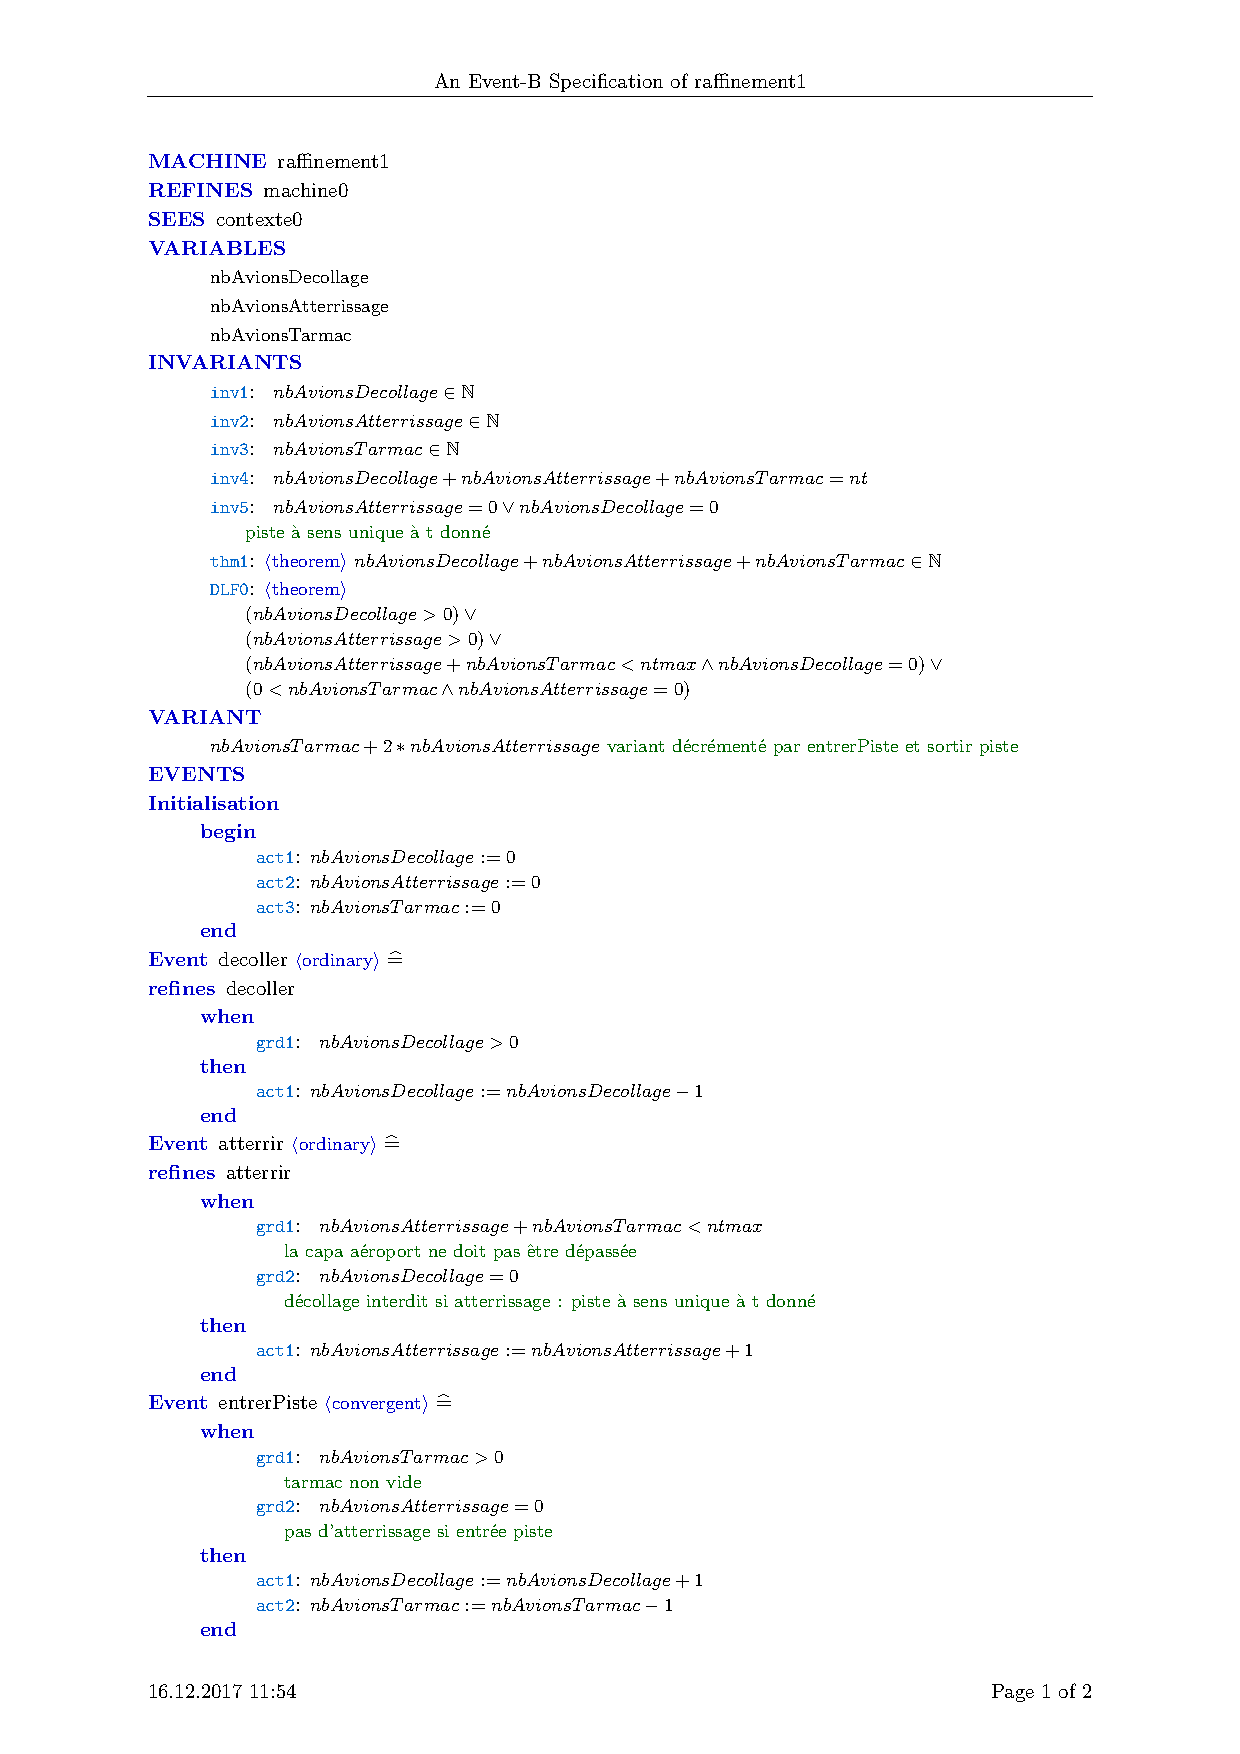
\includegraphics[scale=0.8]{images/1/machine1}
 		\caption{}
 		\label{machine1}
 	\end{center}
 \end{figure}
 
 \subsection{Preuves}
 
 Comme pour la machine abstraite, le théorème DLF0 doit être prouvé interactivement via la perspective "Proving" pour prendre en compte toutes les hypothèses.
 
 \begin{figure}[H]
 	\begin{center}	
 		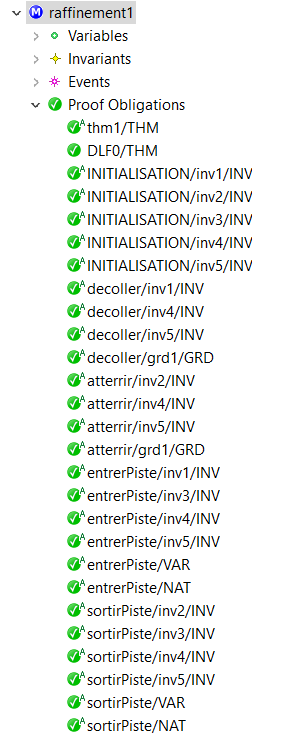
\includegraphics[scale=1.2]{images/1/proof1}
 		\caption{Preuves du premier raffinement}
 		\label{proof1}
 	\end{center}
 \end{figure}
 

 
 




